%!TEX root = mainfile.tex

\subsection{European Extremely Large Telescope} % (fold)
\label{sub:european_extremely_large_telescope}
(Rahim)

	One of a new generation of ground based telescopes, the European Extremely Large Telescope (E-ELT), shown in Figure~\ref{fig:artist_eelt}, is scheduled for first light in 2022 and has a projected lifetime of 30 years, although major upgrades are expected during this period\cite[p.~163]{E_ELT_Construction_Proposal}, and an estimated cost of around 1083\,million Euros. The Telescope will be constructed on Cerro Armazones in Chile at an altitude of approximately \SI{3060}{\metre} and will be part of the La Silla Paranal observatory. With a primary mirror diameter of \SI{39.9}{\metre}, the E-ELT will be the largest optical/near-infrared telescope in the world. The telescope will also incorporate adaptive optics, discussed in Section~\ref{ssub:adaptive_optics}, which will result in it being able to correct for atmospheric perturbations and therefore be diffraction limited.
	\begin{figure}[htbp]
		\centering
		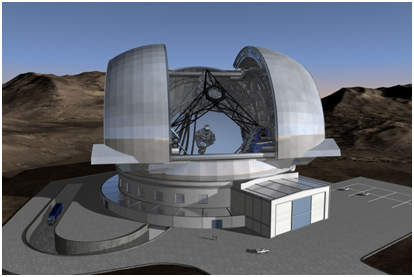
\includegraphics[width=0.6\textwidth]{../Images/E-ELT.png}
		\caption{An artist's impression of the E-ELT\cite{E_ELT_Enclosure}}\label{fig:artist_eelt}
	\end{figure}

	One of the most important components of the E-ELT is the dome within which the telescope is enclosed. This primarily provides protection to the telescope against unfavourable weather conditions and during the day. The dome is designed to allow complete freedom to the telescope, allowing it to position itself, permitting observations between a $20^{\circ}$ angle to the horizon and zenith and also incorporates a windscreen protecting the mirrors. As well as being water-tight, the dome is also air-tight to minimise the air-conditioning load. The E-ELT will use an air-conditioning system to cool the mirror and instrumentation to ensure optimum operating conditions in preparation for the upcoming night.

	The E-ELT utilises a three mirror anastigmat system with two further mirrors providing the adaptive optics, shown below in Figure~\ref{fig:5_mirror_eelt}, with the fifth mirror directing the beam towards the Nasmyth focus\cite[p.~16]{E_ELT_Construction_Proposal}. The primary mirror, measuring \SI{39.3}{\metre} in diameter, will be comprised of 798 hexagonal segments eventually producing a collecting area of \SI{978}{\square\metre}. The E-ELT will therefore have a light collecting power approximately 13 times larger than any existing telescope and is predicted to produce images 16 times sharper than those of the Hubble Space Telescope. Other new generation extremely large telescopes include the Giant Magellan Telescope with a primary mirror of diameter \SI{25}{\metre} and the Thirty Metre Telescope with a primary mirror of diameter \SI{30}{\metre}. The E-ELT however remains the largest of these planned telescopes.
	\begin{figure}[htbp]
		\centering
		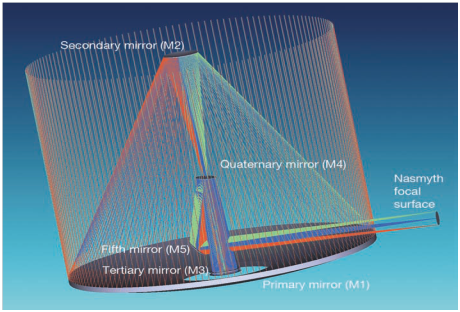
\includegraphics[width=0.6\textwidth]{../Images/Anastigmat.png}
		\caption{The 5 mirror design to be utilised on the E-ELT}\label{fig:5_mirror_eelt}
	\end{figure}

	\subsubsection{Main Aims} % (fold)
	\label{ssub:main_aims}
		One of the main aims of the E-ELT will be the search for extra-solar planets.  This will include the detection of extra-solar planets using the radial velocity technique, the detection of variations of the radial velocity of a star with respect to the Earth in response to the gravity of an orbiting planet, as well as possible direct imaging of larger planets. The E-ELT may also be used to characterise the atmosphere of these larger planets using low resolution spectroscopy. The observation of giant planets in star forming regions and young stellar clusters will also provide an insight into their evolution.

		Another of the main aims is the study of the universe at high redshift. The E-ELT will look back at the earliest galaxies formed after the ``dark ages'', the galaxies therefore responsible for the reionization of the universe. Properties of these early galaxies including their star formation rates, ages, metallicities and stellar masses will be determined contributing to a better understanding of galaxy formation and evolution.

		The E-ELT will also help to understand the nature of dark energy through the discovery and identification of type 1a supernovae. As these are excellent distance indicators, they can be used to map space and its expansion history thus providing information on what is believed to be the source of this expansion. The E-ELT will also attempt to measure small time-drifts in the redshifts of distant objects in the inter-galactic medium, a consequence of the evolution the universal expansion rate. The E-ELT will also attempt to discover variations of physical constants over time which, if found to be the case, will have great consequences on our understanding of the general laws of physics.
	% subsubsection main_aims (end)

	\subsubsection{Instrumentation} % (fold)
	\label{ssub:instrumentation}
		At first light, the E-ELT will have just two instruments\cite{E_ELT_Instrumentation}, a diffraction-limited near-infrared imager (MICADO) as well as a single-field near-infrared wide-band integral field spectrograph (HARMONI). Three further objects, a mid-infrared imager and spectrometer (METIS), a high-resolution spectrometer (SIMPLE) and multi-object spectrometer (OPTIMOS) will be added soon after first light\cite{E_ELT_Instrumentation}. There are also some other concepts being studied for use on the E-ELT including a planet imager with extreme adaptive optics (EPICS). Importantly, the instrumentation available will mean that the E-ELT can be used for both photometry and spectroscopy and is also said to be able to switch between these instruments in a matter of minutes.
	% subsubsection instrumentation (end)
% subsection european_extremely_large_telescope (end)
